\section{Meeting Notes}

\begin{figure}[htbp]
    \centering
    
\includegraphics[width=0.7\textwidth]{figures/Appendix-MeetingNotes/meeting_note_1.png}
    \caption*{Meeting notes from 2024-10-07} 
    \label{fig:meeting1}
    \end{figure}

    \begin{figure}[htbp]
        \centering
        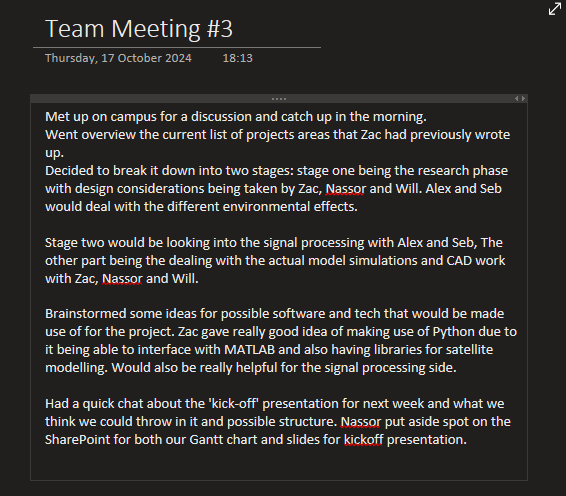
\includegraphics[width=0.7\textwidth]{figures/Appendix-MeetingNotes/meeting_note_3.png}
        \caption*{Meeting notes from 2024-10-17} 
        \label{fig:meeting3}
        \end{figure}

        \begin{figure}[htbp]
            \centering
            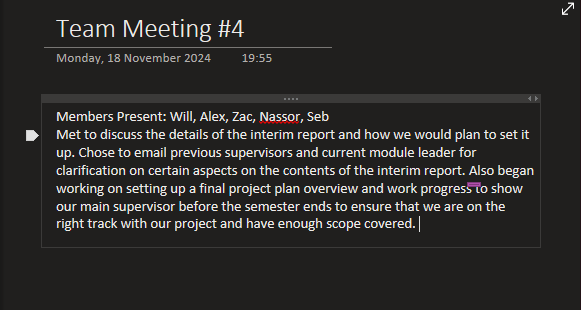
\includegraphics[width=0.7\textwidth]{figures/Appendix-MeetingNotes/meetingnote4.png}
            \caption*{Meeting notes from 2024-11-18} 
            \label{fig:meeting4}
            \end{figure}

            \begin{figure}[htbp]
                \centering
                
\includegraphics[width=0.7\textwidth]{figures/Appendix-MeetingNotes/meeting_note_5.png}
                \caption*{Meeting notes from 2024-11-21} 
                \label{fig:meeting5}
                \end{figure}

                
                \begin{figure}[htbp]
                    \centering
                    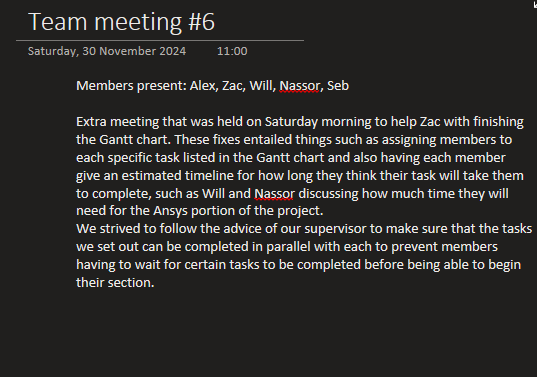
\includegraphics[width=0.7\textwidth]{figures/Appendix-MeetingNotes/meeting_note_6.png}
                    \caption*{Meeting notes from 2024-11-30} 
                    \label{fig:meeting6}
                    \end{figure}

                    
                    \begin{figure}[htbp]
                        \centering
                        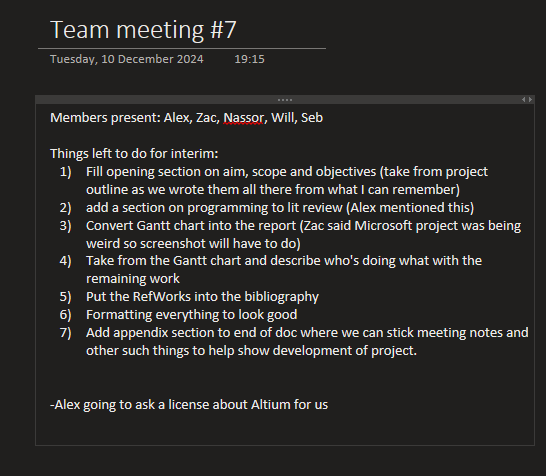
\includegraphics[width=0.7\textwidth]{figures/Appendix-MeetingNotes/meetingnote7.png}
                        \caption*{Meeting notes from 2024-12-10} 
                        \label{fig:meeting7}
                        \end{figure}

                        
                        \begin{figure}[htbp]
                            \centering
                            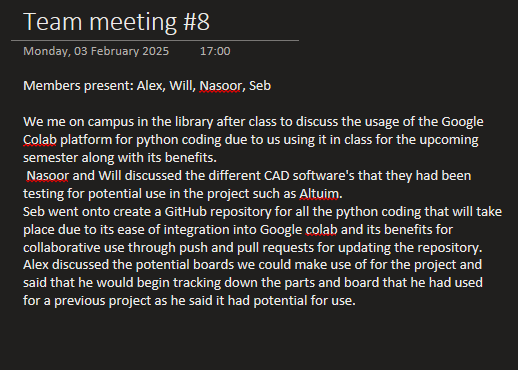
\includegraphics[width=0.7\textwidth]{figures/Appendix-MeetingNotes/meetingnote8.png}
                            \caption*{Meeting notes from 2025-02-03} 
                            \label{fig:meeting8}
                            \end{figure}

                            
                            \begin{figure}[htbp]
                                \centering
                                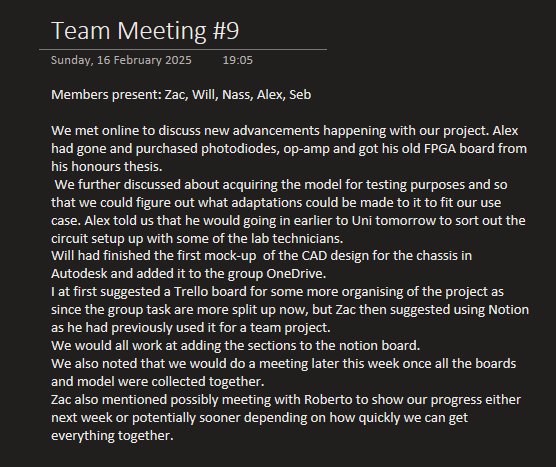
\includegraphics[width=0.7\textwidth]{figures/Appendix-MeetingNotes/meeting9.png}
                                \caption*{Meeting notes from 2025-02-16} 
                                \label{fig:meeting9}
                                \end{figure}

                                
                                \begin{figure}[htbp]
                                    \centering
                                    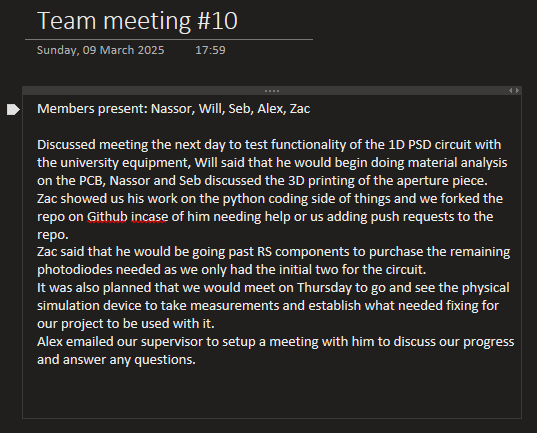
\includegraphics[width=0.7\textwidth]{figures/Appendix-MeetingNotes/meeting10.png}
                                    \caption*{Meeting notes from 2025-03-09} 
                                    \label{fig:meeting10}
                                    \end{figure}

                                    
                                    \begin{figure}[htbp]
                                        \centering
                                        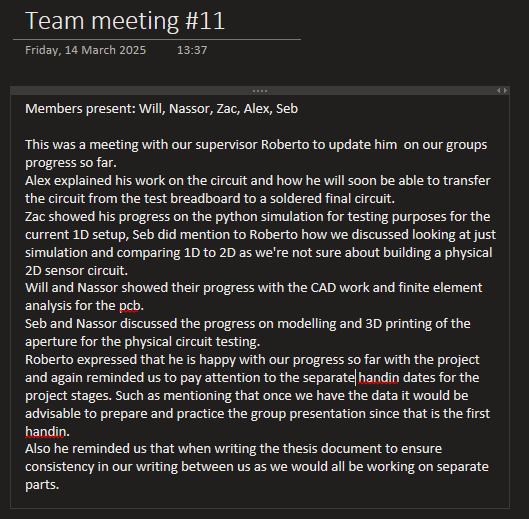
\includegraphics[width=0.7\textwidth]{figures/Appendix-MeetingNotes/meeting_note_11.png}
                                        \caption*{Meeting notes from 2025-03-14} 
                                        \label{fig:meeting11}
                                        \end{figure}

                                        

                                        \begin{figure}[htbp]
                                            \centering
                                            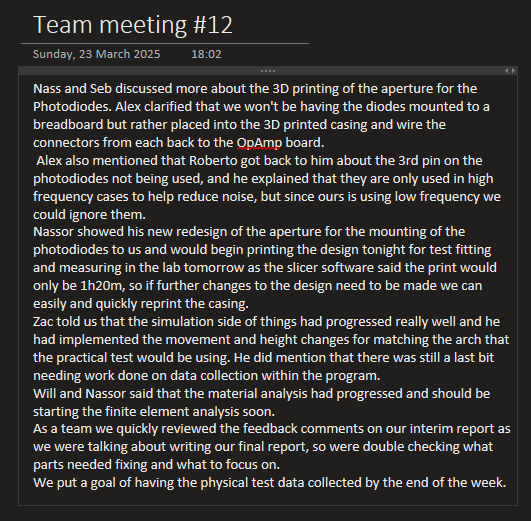
\includegraphics[width=0.7\textwidth]{figures/Appendix-MeetingNotes/meetingNote12.png}
                                            \caption*{Meeting notes from 2025-03-23} 
                                            \label{fig:meeting12}
                                            \end{figure}
                                        
\section{Appendix - RED LED Strip Code}
\subsection{LED Strip Code for automatic transition}
\label{REDappendix}
This code is modified to change the LED position every 5 seconds automatically.


%%% Cpp Code
\begin{lstlisting}[style=cstyle, caption=Cpp Code of the RGB strip with automatic changes, label=lst:RGBcodeAutomatic, language=c++ ]
    #include <FastLED.h>

// LED strip configuration
#define NUM_LEDS 27
#define LED_PIN 5
CRGB leds[NUM_LEDS]; // define FastLED datatype

// automatic transition all leds:
const int timeInterval = 5000;  // miliseconds


// Communication pin from main Arduino
// const int led_status_pin = 12;  // Input pin to receive signals

// LED Positions 
// MODIFY THESE VALUES TO CHANGE PRESET LED POSITIONS

//all positions version
const int NUM_PRESETS = 25;
// modified from 5 positions to all positions automatically every timeInterval seconds
int presetLedPositions[NUM_PRESETS] = {
  1,2,3,4,5,6,7,8,9,10,11,12,13,14,15,16,17,18,19,20,21,22,23,24,25   
};

// State variables
int currentPresetIndex = 2;  // start close to the edge
bool lastSignalState = LOW;

void setup() {
  Serial.begin(9600);
  Serial.println("LED Controller Starting...");
 
  //  LED strip
  FastLED.addLeds<WS2812B, LED_PIN, GRB>(leds, NUM_LEDS);
  FastLED.setBrightness(255);  //  brightness (0-255)
 
  //  communication pin
  // pinMode(led_status_pin, INPUT); not used
 
  // Clear LED
  clearAllLeds();
  
  //  starting position
  currentPresetIndex = 0;  // begining position 
  
  // small delay
  delay(50);
 
  // Show initial LED position on screen
  updateLedDisplay(presetLedPositions[currentPresetIndex]);
  
  // Debug output
  Serial.print("Starting with preset index: ");
  Serial.println(currentPresetIndex);
}

void loop() {

  
  // do not wait for input anymore, automatic
  if (1) {   
    
    // Clear previous LEDs
    clearAllLeds();
    
    // Move to next preset
    currentPresetIndex = (currentPresetIndex + 1) % NUM_PRESETS;
    
    // Update LED display
    updateLedDisplay(presetLedPositions[currentPresetIndex]);
    
    // wait preset speed
    delay(timeInterval);
  }
  

}

void clearAllLeds() {
  for (int i = 0; i < NUM_LEDS; i++) {
    leds[i] = CRGB::Black;
  }
  FastLED.show();
}

// update the location of the LEDS, 
// based on centerindex
void updateLedDisplay(int centerIndex) {
  if (centerIndex > 0) {
    leds[centerIndex - 1] = CRGB::White;
  }
  
  leds[centerIndex] = CRGB::White;
  
  if (centerIndex < NUM_LEDS - 1) {
    leds[centerIndex + 1] = CRGB::White;
  }
  
  FastLED.show();
  Serial.print("LED updated at preset index: ");
  Serial.print(currentPresetIndex + 1);  // Display 1-5 instead of 0-4
  Serial.print(" (LED position: ");
  Serial.print(centerIndex);
  Serial.println(")");
}
\end{lstlisting}

\subsection{LED Strip Code for Manual 5 location transition}
%%% Cpp Code
\begin{lstlisting}[style=cstyle, caption=Cpp Code of the RGB strip with Manual 5 locations, label=lst:RGBcodeManual, language=c++ ]
    #include <FastLED.h>

// LED strip configuration
#define NUM_LEDS 27
#define LED_PIN 5
CRGB leds[NUM_LEDS];

// Communication pin from main Arduino
const int led_status_pin = 12;  // Input pin to receive signals

// Preset LED Positions Configuration
// MODIFY THESE VALUES TO CHANGE PRESET LED POSITIONS
const int NUM_PRESETS = 5;
int presetLedPositions[NUM_PRESETS] = {
  3,    // Position 1 - center LED index
  9,    // Position 2 - center LED index
  13,   // Position 3 - center LED index (middle)
  17,   // Position 4 - center LED index
  23    // Position 5 - center LED index
};

// State variables
int currentPresetIndex = 2;  // Start at center position (index 2, which is the 3rd preset)
bool lastSignalState = LOW;

void setup() {
  Serial.begin(9600);
  Serial.println("LED Controller Starting...");
  
  // Initialize LED strip
  FastLED.addLeds<WS2812B, LED_PIN, GRB>(leds, NUM_LEDS);
  
  // Initialize communication pin
  pinMode(led_status_pin, INPUT);
  
  // Clear all LEDs
  clearAllLeds();
  
  // Show initial LED position
  updateLEDstrip(presetLedPositions[currentPresetIndex]);
}

void loop() {
    // Read signal from main Arduino
    bool signalState = digitalRead(led_status_pin);

    // Apply debounce delay
    delay(5);

    // Read signal again after debounce
    bool debouncedSignalState = digitalRead(led_status_pin);

    // Only proceed if the signal is stable
    if (debouncedSignalState == signalState) {
        // If stable signal state changed from previous loop iteration
        if (debouncedSignalState != lastSignalState) {
            // Debug print for any signal change
            Serial.print("Signal changed from ");
            Serial.print(lastSignalState ? "HIGH" : "LOW");
            Serial.print(" to ");
            Serial.println(debouncedSignalState ? "HIGH" : "LOW");
            
            // Detect rising edge (LOW to HIGH transition)
            if (debouncedSignalState == HIGH && lastSignalState == LOW) {
            Serial.println("Signal received from main Arduino");
            
            // Clear previous LEDs
            clearAllLeds();
            
            // Move to next preset
            currentPresetIndex = (currentPresetIndex + 1) % NUM_PRESETS;
            
            // Update LED srip
            updateLEDstrip(presetLedPositions[currentPresetIndex]);
            }
        }

        // Update the last signal state
        lastSignalState = debouncedSignalState;
        }
    // If signal is not stable after debounce, don't update lastSignalState
    }

void clearAllLeds() {
  for (int i = 0; i < NUM_LEDS; i++) {
    leds[i] = CRGB::Black;
  }
  FastLED.show();
}

void updateLEDstrip(int centerIndex) {
  
  if (centerIndex > 0) {
    leds[centerIndex - 1] = CRGB::White;
  }
  
  leds[centerIndex] = CRGB::White;
  
  if (centerIndex < NUM_LEDS - 1) {
    leds[centerIndex + 1] = CRGB::White;
  }
  
  FastLED.show();
  Serial.print("LED updated at preset index: ");
  Serial.print(currentPresetIndex + 1); 
  Serial.print(" (LED position: ");
  Serial.print(centerIndex);
  Serial.println(")");
}
\end{lstlisting}


 
\subsection{ARCH controller C++ code }
%%% Cpp code
\begin{lstlisting}[style=cstyle, caption=C++ Code of the ARCH Arduino, label=lst:ArchCode, language=c++ ]
#include <Servo.h>
#include <LiquidCrystal_I2C.h>

// Servo 
Servo arch_left;
Servo arch_right;

// LCD screen
LiquidCrystal_I2C lcd(0x27, 16, 2);

// Pin Definitions
const int pushButton = 13;
const int led_status_pin = 12;  // Signal to secondary Arduino for LED control

// Presets  

const int NUM_PRESETS = 5;
int presetAngles[NUM_PRESETS] = {
  20,   // Position 1 - angle in degrees
  50,   // Position 2 - angle in degrees
  90,   // Position 3 - angle in degrees (center) - may not reach, due to servos?
  130,  // Position 4 - angle in degrees
  160   // Position 5 - angle in degrees
};

// State Variables
int current_index = 2;  // Start at center position (index 2, which is the 3rd preset)
bool lastButtonState = HIGH; // Using INPUT_PULLUP, so HIGH is not pressed

void setup() {
  Serial.begin(9600);
  
  // Initialize servos
  arch_left.attach(5);
  arch_right.attach(6);
  
  // Set initial position
  change_state(current_index);
  
  // Initialize LED communication pin
  pinMode(led_status_pin, OUTPUT);
  digitalWrite(led_status_pin, LOW);
  
  // Initialize LCD
  lcd.init();
  lcd.backlight();
  updateDisplay();
  
  // Initialize button
  pinMode(pushButton, INPUT_PULLUP);
}

void loop() {
  // Read button state
  bool buttonState = digitalRead(pushButton);
  
  // Check for button press (transition from HIGH to LOW)
  if (buttonState == LOW && lastButtonState == HIGH) {
    // Move to next preset
    current_index = (current_index + 1) % NUM_PRESETS;
    
    // Update servo position
    change_state(current_index);
    
    // Update display
    updateDisplay();
    
    // Signal the LED Arduino to change LEDs
    signalLedArduino();
    
    // Debounce delay
    delay(200);
  }
  
  // Save button state for next iteration
  lastButtonState = buttonState;
}

void change_state(int presetIndex) {
  // do a calibration each time to ensure correct position
  arch_left.write(0);
  arch_right.write(180); // Mirror  (180 - 0)
  
  // add delay to reach location
  delay(5000);  // Adjust delay as needed for your servos

  int angle = presetAngles[presetIndex];
  
  // Update servos with the new location
  arch_left.write(angle);
  arch_right.write(180 - angle); // Mirror movement
  // debug
  Serial.print("Moving to preset ");
  Serial.print(presetIndex + 1);
  Serial.print(" (angle: ");
  Serial.print(angle);
  Serial.println(" degrees)");
}

void signalLedArduino() {
  // Trigger the RGB Arduino's LED change
  digitalWrite(led_status_pin, HIGH);
  delay(50);  // Brief pulse to trigger the other Arduino and pass debounce check
  digitalWrite(led_status_pin, LOW);
  
  Serial.println("Sent signal to LED Arduino");
}

void updateDisplay() {
  lcd.clear();
  lcd.setCursor(0, 0);
  lcd.print("Position: ");
  lcd.print(current_index + 1);  
  
  lcd.setCursor(0, 1);
  lcd.print("Alt:");
  lcd.print(presetAngles[current_index]);
  lcd.print(" Az:");
  lcd.print(presetAngles[current_index]);
}
\end{lstlisting}
